\documentclass{article}
\usepackage{algorithm}
\usepackage{algpseudocodex}
\usepackage{graphicx}
\usepackage{amsmath}
\usepackage{bm}
\usepackage{array}
\title{CSEP501 : Compiler Construction: Homework 3}
\author{Karuna Sagar Krishna}

\begin{document}
    \maketitle

    \section*{Question 1}

    \subsection*{1a}
    Adding production rule for $E'$ and number all the production rules, we have:
    \begin{center}
        \begin{tabular}{ l l }
        \hline
        rule \# & production \\
        \hline
        0   &   $E'$  ::= \textit{E \$} \\
        1   &   E   ::= \textit{D} \\
        2   &   D   ::= \textit{T} \\
        3   &   D   ::= \textit{S} \\
        4   &   S   ::= \textit{T like A} \\
        5   &   T   ::= \textit{quick} \\
        6   &   T   ::= \textit{strong} \\
        7   &   A   ::= \textit{bunny} \\
        8   &   A   ::= \textit{ox} \\
        \end{tabular}
    \end{center}

    Using the closure, goto and LR(0) construction algorithms, we get the following DFA for viable prefixes:
    \begin{figure}[H]
        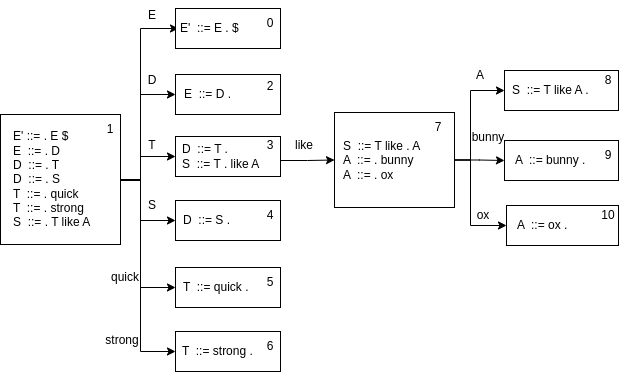
\includegraphics[width=1\textwidth]{hw3-1a.png}
    \end{figure}

    The LR(0) parsing table built using the above DFA and parse table construction algorithms is as follows:
    \begin{center}
        \begin{tabular}{ c c c c c c c | c c c c c }
            \hline
            & like & quick & strong & bunny & ox & \$ & E & D & T & S & A \\
            \hline
            0 & & & & & & acc & \\
            1 & & s5 & s6 & & & & g0 & g2 & g3 & g4 & \\
            2 & r1 & r1 & r1 & r1 & r1 & r1 & \\
            3 & s7,r2 & r2 & r2 & r2 & r2 & r2 & \\
            4 & r3 & r3 & r3 & r3 & r3 & r3 & \\
            5 & r5 & r5 & r5 & r5 & r5 & r5 & \\
            6 & r6 & r6 & r6 & r6 & r6 & r6 & \\
            7 & & & & s9 & s10 & & & & & & g8 \\
            8 & r4 & r4 & r4 & r4 & r4 & r4 & \\
            9 & r7 & r7 & r7 & r7 & r7 & r7 & \\
            10 & r8 & r8 & r8 & r8 & r8 & r8 & \\
        \end{tabular}
    \end{center}
    
    \subsection*{1b}
    \begin{center}
        \begin{tabular}{ c c l l }
            \hline
            & nullable & FIRST & FOLLOW \\
            \hline
            E & no & \{quick, strong\} & \{\$\} \\
            D & no & \{quick, strong\} & \{\$\} \\
            T & no & \{quick, strong\} & \{like, \$\} \\
            S & no & \{quick, strong\} & \{\$\} \\
            A & no & \{bunny, ox\} & \{\$\} \\
        \end{tabular}
    \end{center}
    
    \subsection*{1c}
    \begin{center}
        \begin{tabular}{ c c c c c c c | c c c c c }
            \hline
            & like & quick & strong & bunny & ox & \$ & E & D & T & S & A \\
            \hline
            0 & & & & & & acc & \\
            1 & & s5 & s6 & & & & g0 & g2 & g3 & g4 & \\
            2 & & & & & & r1 & \\
            3 & s7 & & & & & r2 & \\
            4 & & & & & & r3 & \\
            5 & r5 & & & & & r5 & \\
            6 & r6 & & & & & r6 & \\
            7 & & & & s9 & s10 & & & & & & g8 \\
            8 & & & & & & r4 & \\
            9 & & & & & & r7 & \\
            10 & & & & & & r8 & \\
        \end{tabular}
    \end{center}

    \subsection*{1d}
    From the LR(0) table we can see that there is a shift reduce conflict at state 3 for terminal $like$. Because of this the grammar is not LR(0).

    The grammar is SLR because we can resolve the shift reduce conflict by using the FIRST and FOLLOW sets as shown in the above SLR parse table.
    
    \section*{Question 2}
    \begin{center}
        \begin{tabular}{ l l }
        \hline
        rule \# & production \\
        \hline
        1   &   A   ::= \textit{s C n g} \\
        2   &   A   ::= $\epsilon$ \\
        3   &   B   ::= \textit{C r} \\
        4   &   B   ::= \textit{t} \\
        5   &   C   ::= \textit{B i} \\
        6   &   C   ::= \textit{t} \\
        \end{tabular}
    \end{center}

    \begin{center}
        \begin{tabular}{ c c l l }
            \hline
            & nullable & FIRST & FOLLOW \\
            \hline
            A & yes & \{s\} & \{\$\} \\
            B & no & \{t\} & \{\i\} \\
            C & no & \{t\} & \{r, n\} \\
        \end{tabular}
    \end{center}

    Lets consider non-terminal $B$ which has two production rules $B ::= C r$ and $B ::= t$. Here neither of the productions step into $\epsilon$, so $FIRST(C r) \cap FIRST(t)$ should be empty for the grammar to satisfy LL(1) property. Clearly, $FIRST(t) = \{t\}$ and $FIRST(C) \in FIRST(C r)$, so we see $FIRST(C) \cap FIRST(t) \neq \emptyset$.

    Similarly, for non-terminal $C$, $FIRST(B i) \cap FIRST(t) = FIRST(B) \cap FIRST(t) \neq \emptyset$. So the grammar is not LL(1).

    There is an indirect left recursion between $B$ and $C$. So we substitute $B$ in $C$ production rules to make this is a direct left recursion. We can eliminate $B$ production rules since $B$ is no longer referenced anywhere; note, this is not possible if we replaced $C$ in $B$ since it shows up in $A$ production rules. We get the following grammar:

    \begin{center}
        \begin{tabular}{ l l }
        \hline
        rule \# & production \\
        \hline
        1   &   A   ::= \textit{s C n g} \\
        2   &   A   ::= $\epsilon$ \\
        3   &   C   ::= \textit{C r i} \\
        4   &   C   ::= \textit{t i} \\
        5   &   C   ::= \textit{t} \\
        \end{tabular}
    \end{center}

    Now we have direct left recursion in $C$, using the formal left recursion solution to eliminate it, we get:

    \begin{center}
        \begin{tabular}{ l l }
        \hline
        rule \# & production \\
        \hline
        1   &   A   ::= \textit{s C n g} \\
        2   &   A   ::= $\epsilon$ \\
        3   &   C   ::= \textit{t i $C'$} \\
        4   &   C   ::= \textit{t $C'$} \\
        5   &   $C'$  ::= \textit{r i $C'$} \\
        6   &   $C'$  ::= $\epsilon$ \\
        \end{tabular}
    \end{center}

    Here we see common prefix on RHS of $C$ production rules. Using the left factor removal solution, we get:

    \begin{center}
        \begin{tabular}{ l l }
        \hline
        rule \# & production \\
        \hline
        1   &   A   ::= \textit{s C n g} \\
        2   &   A   ::= $\epsilon$ \\
        3   &   C   ::= \textit{t $C''$} \\
        3   &   $C''$   ::= \textit{i $C'$} \\
        4   &   $C''$   ::= \textit{$C'$} \\
        5   &   $C'$  ::= \textit{r i $C'$} \\
        6   &   $C'$  ::= $\epsilon$ \\
        \end{tabular}
    \end{center}

    Recalculating the FIRST and FOLLOW sets, we get:

    \begin{center}
        \begin{tabular}{ c c l l }
            \hline
            & nullable & FIRST & FOLLOW \\
            \hline
            A & yes & \{s\} & \{\$\} \\
            C & no & \{t\} & \{n\} \\
            $C''$ & yes & \{i, r\} & \{n\} \\
            $C'$ & yes & \{r\} & \{n\} \\
        \end{tabular}
    \end{center}

    Now, lets consider all non-terminals and verify the LL(1) property on them.

    For non-terminal $A$, there are 2 production rules and since one of the production steps to $\epsilon$, we check for $FIRST(s C n g) \cap FOLLOW(A) = \emptyset$. Clearly, $FIRST(s C n g) = \{s\}$, so the LL(1) property holds.

    For non-terminal $C$, there is only one production rule hence it is deterministic. Hence LL(1) property holds trivially.

    For non-terminal $C''$, there are 2 production rules and neither of them steps into $\epsilon$. So the LL(1) property to verify is $FIRST(i C') \cap FIRST(C') = \emptyset$. $FIRST(i C') = \{i\}$ and $FIRST(C') = \{r\}$, so the LL(1) property holds.

    For non-terminal $C'$, there are 2 production rules and one of them steps into $\epsilon$. So we should verify $FIRST(r i C') \cap FOLLOW(C') = \emptyset$. $FIRST(r i C') = \{r\}$ and $FOLLOW(C') = \{n\}$, so the LL(1) property holds.

    Since the LL(1) property holds for every non-terminal, the new transformed grammar is LL(1).

    \section*{Question 3}
    \begin{center}
        \begin{tabular}{ l l }
        \hline
        rule \# & production \\
        \hline
        1   &   S   ::= \textit{S ; S} \\
        2   &   S   ::= \textit{id := E} \\
        3   &   S   ::= \textit{print ( L )} \\
        4   &   E   ::= \textit{id} \\
        5   &   E   ::= \textit{num} \\
        6   &   E   ::= \textit{E + E} \\
        7   &   E   ::= \textit{( S , E )} \\
        8   &   L   ::= \textit{E} \\
        9   &   L   ::= \textit{L , E} \\
        \end{tabular}
    \end{center}

    We have seen rule 6 in class, where we saw that it was part of ambiguous grammar. Specifically, it doesn't clarify the associativity of the $+$ operator. Similarly, rule 1 has a similar structure to rule 6, so it must have the same ambiguity. This can be seen by the following 2 left most derivation leading to the same target sentence $id := num ; id := num ; id := num$:

    \begin{align*}
        S   & \rightarrow S ; S \\
            & \rightarrow S ; S ; S \\
            & \rightarrow id := E ; S ; S \\
            & \rightarrow id := num ; S ; S \\
            & \rightarrow id := num ; id := E ; S \\
            & \rightarrow id := num ; id := num ; S \\
            & \rightarrow id := num ; id := num ; id := E \\
            & \rightarrow id := num ; id := num ; id := num \\
    \end{align*}

    \begin{align*}
        S   & \rightarrow S ; S \\
            & \rightarrow id := E ; S \\
            & \rightarrow id := num ; S \\
            & \rightarrow id := num ; S ; S \\
            & \rightarrow id := num ; id := E ; S \\
            & \rightarrow id := num ; id := num ; S \\
            & \rightarrow id := num ; id := num ; id := E \\
            & \rightarrow id := num ; id := num ; id := num \\
    \end{align*}

    Since the same target sentence/string has 2 different left most derivations, the grammar is ambiguous.

    Lets assume, we want to have left associativity for $;$ and $+$ operators. To achieve this we want to have only left recursion so that the parse tree leans on the left thereby honoring left associativity eg. consider $id + id + id$, with left recursion we would be forced to evaluate the left $+$ first i.e. $(id + id) + id$. This implies a production rule that looks like $E ::= E + E$ gets transformed to $E ::= E + T | T$, similar to what we saw with classic expression grammar in class (lecture 2). Applying this to the above grammar, leads to:

    \begin{center}
        \begin{tabular}{ l l }
        \hline
        rule \# & production \\
        \hline
        1   &   S   ::= \textit{S ; $S'$} \\
        2   &   S   ::= \textit{$S'$} \\
        3   &   $S'$  ::= \textit{id := E} \\
        4   &   $S'$  ::= \textit{print ( L )} \\
        5   &   E   ::= \textit{E + $E'$} \\
        6   &   E   ::= \textit{$E'$} \\
        7   &   $E'$  ::= \textit{id} \\
        8   &   $E'$  ::= \textit{num} \\
        9   &   $E'$  ::= \textit{( S , E )} \\
        10  &   L   ::= \textit{E} \\
        11  &   L   ::= \textit{L , E} \\
        \end{tabular}
    \end{center}

    This grammar doesn't seem to be ambiguous. However, this is not LL(1) grammar since it has left recursion on $S$, $E$ and $L$. Using the formal left recursion solution, we transform the grammar to:

    \begin{center}
        \begin{tabular}{ l l }
        \hline
        rule \# & production \\
        \hline
        1   &   S   ::= \textit{$S'$ $S''$} \\
        2   &   $S''$ ::= \textit{; $S'$ $S''$} \\
        3   &   $S''$ ::= $\epsilon$ \\
        4   &   $S'$  ::= \textit{id := E} \\
        5   &   $S'$  ::= \textit{print ( L )} \\
        6   &   E   ::= \textit{$E'$ $E''$} \\
        7   &   $E''$ ::= \textit{+ $E'$ $E''$} \\
        8   &   $E''$ ::= $\epsilon$ \\
        9   &   $E'$  ::= \textit{id} \\
        10  &   $E'$  ::= \textit{num} \\
        11  &   $E'$  ::= \textit{( S , E )} \\
        12  &   L   ::= \textit{E $L''$} \\
        13  &   $L''$ ::= \textit{, E $L''$} \\
        14  &   $L''$ ::= $\epsilon$ \\
        \end{tabular}
    \end{center}

    This transformed grammar does not have left recursion or common prefix on RHS of production rules. Calculating the FIRST and FOLLOW sets, we get:

    \begin{center}
        \begin{tabular}{ c c l l }
            \hline
            & nullable & FIRST & FOLLOW \\
            \hline
            S & no & \{id print\} & \{, \$\} \\
            $S''$ & yes & \{;\} & \{, \$\} \\
            $S'$ & no & \{id print\} & \{; , \$\} \\
            E & no & \{id num (\} & \{, ) ; \$\} \\
            $E''$ & yes & \{+\} & \{, ) ; \$\} \\
            $E'$ & no & \{id num (\} & \{, + ) ; \$\} \\
            L & no & \{id num (\} & \{)\} \\
            $L''$ & yes & \{,\} & \{)\} \\
        \end{tabular}
    \end{center}

    Now, lets consider all non-terminals and verify the LL(1) property on them.

    There is only one production rule for non-terminals $S$, $E$ and $L$. So the LL(1) property holds trivially.

    \begin{center}
        \begin{tabular}{m{3em} m{25em}}
            $S''$ & since one of the production rules steps into $\epsilon$, we see that $FIRST(; S' S'') \cap FOLLOW(S'') = \{;\} \cap FOLLOW(S'') = \emptyset$. Hence the LL(1) property holds \\ \\
            $S'$ & $FIRST(id := E) \cap FIRST(print (L)) = \{id\} \cap \{print\} = \emptyset$ \\ \\
            $E''$ & since one of the production rules steps into $\epsilon$, we see that $FIRST(+ E' E'') \cap FOLLOW(E'') = \{+\} \cap FOLLOW(E'') = \emptyset$. \\ \\
            $E'$ & $FIRST(id) \cap FIRST(num) = \emptyset$ \\ \\
            $L''$ & since one of the production rules steps into $\epsilon$, we see that $FIRST(, E L'') \cap FOLLOW(L'') = \{,\} \cap FOLLOW(L'') = \emptyset$. \\ \\
        \end{tabular}
    \end{center}

    Hence the grammar is LL(1).
    
\end{document}
